\section*{Результати з математики}
\addcontentsline{toc}{section}{Результати з математики}

Оглянемо отримані $122\ 026$ результатів, при цьому зауважимо, що чоловічих на $11\ 984$ більше за жіночих. 
Зобразимо гістограми результатів ЗНО з математики 2019 року для вибірки, наприклад, $10\ 000$ учнів:

\begin{figure}[H]
    \center{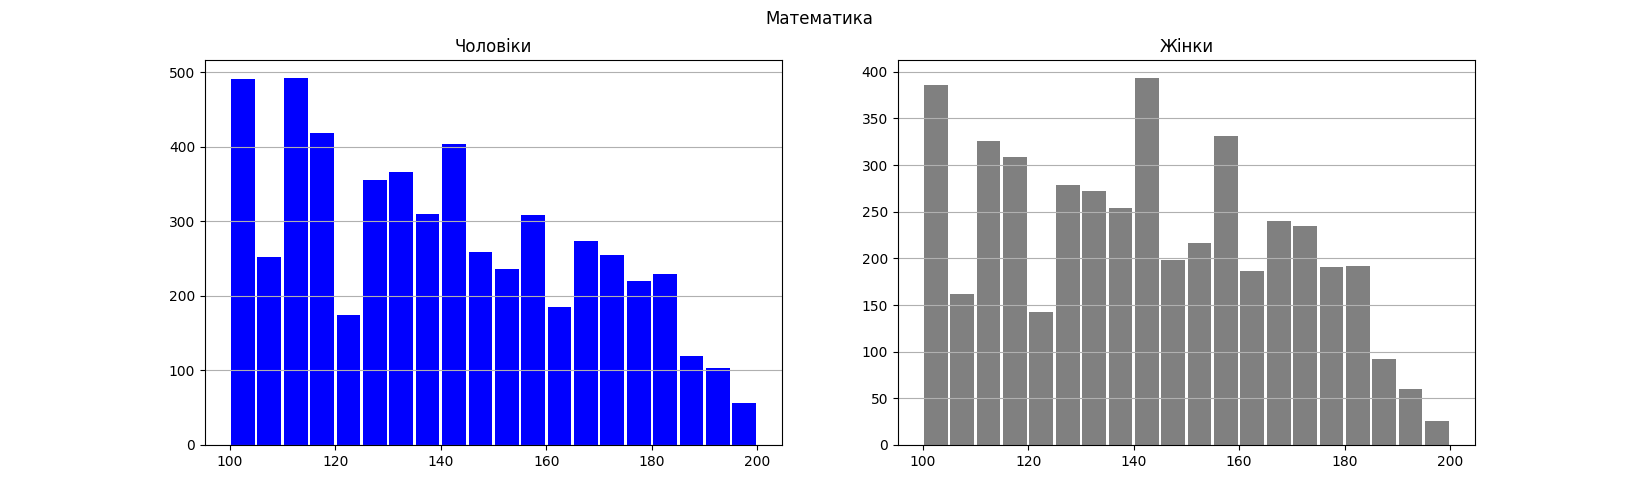
\includegraphics[trim=4cm 0cm 4cm 1cm, clip, width=1\linewidth]{MATH figures/MATH_10000.png}}
    \caption{Результати з математики}
    \label{fig:MATH initial data}
\end{figure}

З'ясуємо, чи відмінність між результатами з математики для жінок та чоловіків є статистично значущою.

\subsection*{Перевірка гіпотези однорідності даних}
\addcontentsline{toc}{subsection}{Перевірка гіпотези однорідності даних}

Нехай маємо дві незалежні вибірки $\left\{ X_i \right\}$ та $\left\{ Y_j \right\}$ однаково розподілених 
випадкових величин, розподіли $F_x$ й $F_y$ яких нам невідомі:
\begin{align*}
    &X_1 \ldots X_n\sim F_x && \text{результати чоловіків} \\
    &Y_1 \ldots Y_m\sim F_y && \text{результати жінок}
\end{align*}

Перевіримо гіпотезу про однорідність статистичного матеріалу, тобто гіпотезу, що ймовірності 
спостереження умовно високих, помірних та низьких балів в обох вибірках є однаковими. Таким чином 
матимемо $k=2$ вибірок, в яких елементи приймають $s=3$ різних значень. За аналогічних позначень гiпотеза 
перевiрки однорiдностi спосережуваних даних формулюватиметься так само як і у виразах~(\ref{formula: hypothesis}):
\begin{align*}
    &\text{нульова гіпотеза} &&H_0: p_{11}=p_{21},\ p_{12}=p_{22},\ p_{13}=p_{23} \\
    &\text{проти альтернативи} && H_1: \exists i,j\quad p_{1,j}\neq p_{2,j}
\end{align*}

А тоді критерієм перевірки гіпотези рівно як і у випадку обробки результатів з 
української мови (\ref{formula: criterion}) слугуватиме правило
\begin{equation*}
    \delta(x_1\ldots x_n,\ y_1\ldots y_m)=
    \begin{cases}
    H_1, & \rho\geqslant\chi^2_{1-\alpha;\ (k-1)(s-1)} \\
    H_0, & \rho<\chi^2_{1-\alpha;\ (k-1)(s-1)} \\
    \end{cases}\ ,
\end{equation*}

де статистика критерію $\rho$ обчислюється аналогічно до формули (\ref{formula: criterion statistics}):
\begin{equation*}
    \rho\equiv \rho(x_1\ldots x_n,\ y_1\ldots y_m)=(n+m)\left( \sum\limits_{i=1}^k \sum\limits_{j=1}^s 
    \frac{\vartheta_{ij}^2}{\vartheta_{i\cdot}\vartheta_{\cdot j}} - 1\right)
\end{equation*}

\subsubsection*{Таблиця спостережуваних даних}
\addcontentsline{toc}{subsubsection}{Таблиця спостережуваних даних}

Складемо таблицю за спостережуваними даними навмання обраних $n=500$ та $m=500$ елементів із вибірок 
результатів ЗНО з математики для чоловіків та жінок:

\begin{table}[H]
    \vspace*{0.8cm}
    \begin{center}
        \begin{tabular}{|c||c|c|c|c|}
            \hline
             & \text{Низькі бали} & \text{Помірні бали} & \text{Високі бали} & \text{Всього} \\
            \hline \hline
            \text{Чоловіки} & 270 & 165 & 65 & 500 \\
            \hline
            \text{Жінки} & 268 & 174 & 58 & 500 \\
            \hline
            \text{Всього} & 538 & 339 & 123 & 1000 \\
            \hline
        \end{tabular}
        \caption{Таблиця спостережуваних значень}
        \label{table: MATH homogeneity data}
    \end{center}
\end{table}

Обчислимо значення статистики критерію:
\begin{equation*}
    \rho = 1000\left( \frac{270^2}{538\cdot 500}+\frac{165^2}{339\cdot 500} + \ldots + 
    \frac{174^2}{339\cdot 500}+\frac{58^2}{123\cdot 500} - 1 \right) = 0.64
\end{equation*}

Водночас на рівні значущості $\alpha=0.01$ значення критичної точки
\begin{equation*} 
    \chi^2_{0.99;\ (2-1)(3-1)}=\chi^2_{0.99;\ 2}=9.21
\end{equation*}

\subsubsection*{Висновок}
\addcontentsline{toc}{subsubsection}{Висновок}

Оскільки значення статистики критерію є меншим за значення критичної точки, то згідно критерію гіпотеза 
про однорідність статистичних даних приймається. Отже, ймовірності спостереження оцінок різного рівня у 
вибірках для чоловіків та жінок, відповідно, є однаковими. Тобто стать ніяким чином не впливає на рівень 
отриманого балу.

\subsubsection*{Значення \texttt{p-value}}
\addcontentsline{toc}{subsubsection}{Значення \texttt{p-value}}

Нехай випадкова величина $\tau$ має такий самий розподіл як і статистика критерію й при цьому не залежить 
від неї: $\tau\sim\chi^2(2)$. Тоді величина \texttt{p-value} обчислюється як така ймовірність:
\[ P(\tau>\rho\ |\ H_0)=P(\tau>0.64)=1-P(\tau\leqslant0.64)=1-F_{\tau}(0.64)=0.7261 \]

Тож для довільних значень $\alpha<\texttt{p-value}$ гіпотеза $H_0$ приймається.

\subsection*{Побудова довірчого інтервалу для різниці середніх}
\addcontentsline{toc}{subsection}{Побудова довірчого інтервалу для різниці середніх}

Маємо дві незалежні вибірки $\left\{ X_i \right\}$ та $\left\{ Y_j \right\}$ 
однаково розподілених випадкових величин, розподіли $F_x$ й $F_y$ яких нам невідомі:
\begin{align*}
    &X_1 \ldots X_n\sim F_x && \text{результати чоловіків} \\
    &Y_1 \ldots Y_m\sim F_y && \text{результати жінок}
\end{align*}

Спробуємо оцінити, в якому інтервалі лежить значення різниці середніх балів для вибірок результатів ЗНО з 
математики чоловіків та жінок.

\subsubsection*{Нормалізація даних та пошук центральної статистики}
\addcontentsline{toc}{subsubsection}{Нормалізація даних та пошук центральної статистики}

Проведемо нормалізацію даних крок за кроком, як це зображено на схемі (\ref{formula: normalization scheme}). 
У результаті отримаємо такі знормовні вибірки:
\begin{align*}
    &\overline{X^1}\ldots \overline{X^N}\sim N(\mu_x,\tfrac{1}{n}\sigma_x^2) && \text{середні результати чоловіків,} \\
    &\overline{Y^1}\ldots \overline{Y^N}\sim N(\mu_y,\tfrac{1}{n}\sigma_y^2) && \text{середні результати жінок,}
\end{align*}

при цьому
\[ \overline{X^i}=\frac{1}{n}\sum\limits_{j=1}^nX_j,\ \overline{Y^i}=\frac{1}{n}\sum\limits_{j=1}^nY_j,\ i=\overline{1,N} \]

Побудуємо гістограми отриманих вибірок та переконаємося, що вони справді мають нормальний розподіл:

\begin{figure}[H]
    \center{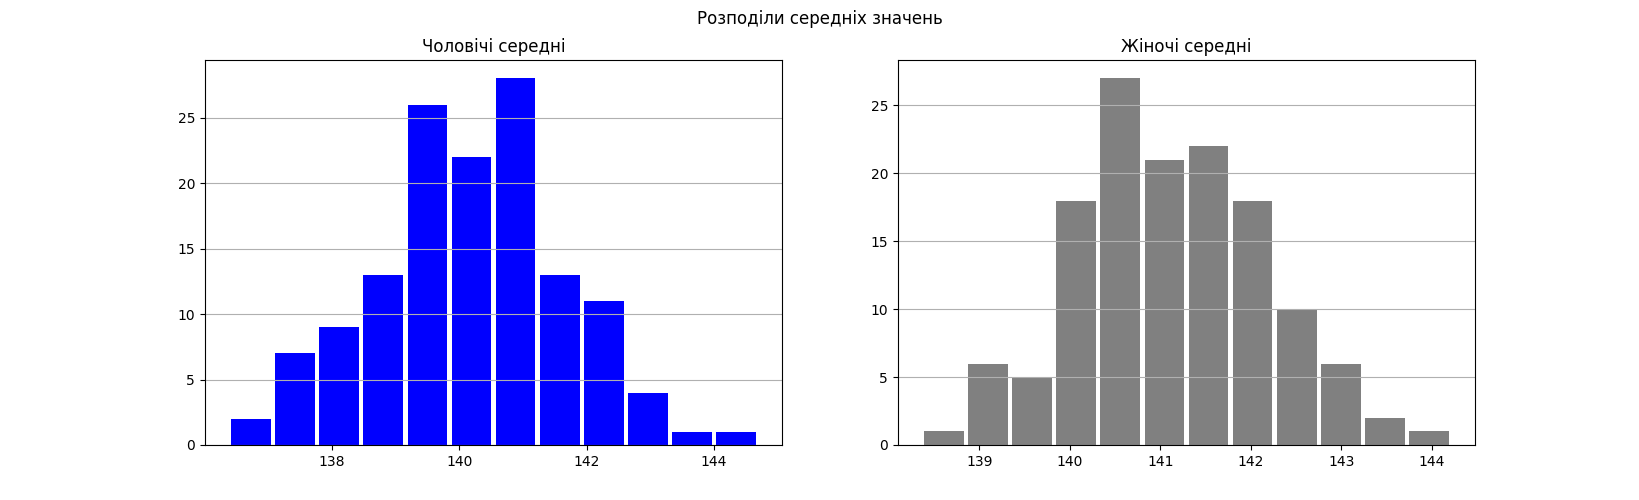
\includegraphics[trim=4cm 0cm 4cm 1cm, clip, width=1\linewidth]{MATH figures/Randomized_means_distribution_m400_N137_v4.png}}
    \caption{Гістограми наборів усереднених результатів ЗНО з математики}
    \label{fig:MATH means data}
\end{figure}

Як бачимо, криві в обох випадках мають схожі риси. Тож знову висунемо припущення, що дисперсії цих вибірок 
однакові, тобто $\sigma_x^2=\sigma_y^2=\sigma^2$. Таким чином: 
\begin{equation*}
    \overline{X^1}\ldots \overline{X^N}\sim N(\mu_x,\tfrac{1}{n}\sigma^2),\ 
    \overline{Y^1}\ldots \overline{Y^N}\sim N(\mu_x,\tfrac{1}{n}\sigma^2)
\end{equation*}

Тоді виконавши аналогічні перетворення, які наведенні на стр. \pageref{seaching central statistic}, 
отримаємо шукану центральну статистику для параметра $\theta=\mu_y-\mu_x:$
\begin{equation*}
    G=\left((\overline{Y}-\overline{X})-\theta\right)\cdot 
    \sqrt{\frac{N^2n}{S_X^2+S_Y^2}}\sim t\left(2N(n-1)\right)
\end{equation*}

\subsubsection*{Побудова довірчого інтервалу}
\addcontentsline{toc}{subsubsection}{Побудова довірчого інтервалу}

Побудуємо довірчий інтервал рівня довіри $\gamma=0.95:$
\[ \gamma \overset{\mathrm{def}}{=} P(g_1<G<g_2)=\int\limits_{g_1}^{g_2}f_G(x)\ dx  \] 

В силу симетричності розподілу Ст'юдента, найкоротший центральний довірчий інтервал матиме вид:
\begin{equation*}
    \gamma = P(g_1<G<g_2)=P(|G|<g),
\end{equation*}
де значення $g=t_{\tfrac{1+\gamma}{2};\ 2N(n-1)}$ -- квантиль рівня $\frac{1+\gamma}{2}$ розподілу Ст'юдента із 
$2N(n-1)$ степенями свободи. Отже:
\begin{equation}
    \gamma = P\left(-t_{\tfrac{1+\gamma}{2};\ 2N(n-1)} < \left((\overline{Y}-\overline{X})-\theta\right)\cdot 
    \sqrt{\frac{N^2n}{S_X^2+S_Y^2}} < t_{\tfrac{1+\gamma}{2};\ 2N(n-1)}\right) \label{formula: MATH trusted interval}
\end{equation}

Останнім кроком вкажемо конкретні значення усіх необхідних величин:

\vspace{0.8cm}
\begin{table}[H]
    \begin{center}
        \begin{tabular}{||c|c|c|c|c|c||}
            \hline
            $n$ & $N$ & $g=t_{0.975;\ 2N(n-1)}$ & $S_X^2$ & $S_Y^2$ & $\overline{Y}-\overline{X}$ \\
            \hline \hline
            400 & 137 & 1.96 & 95092.9605 & 90122.9510 & 0.9639 \\
            \hline
        \end{tabular}
        \caption{Значення шуканих параметрів}
        \label{table: MATH interval}
    \end{center}
\end{table}

Підставивши у вираз (\ref{formula: MATH trusted interval}) значення, які наведені у таблиці вище, отримаємо такий довірчий 
інтервал для параметра $\theta=\mu_y-\mu_x$:
\begin{equation*}
    P(0.66 < \theta < 1.27)=0.95
\end{equation*}

\newpage
\subsubsection*{Висновок}
\addcontentsline{toc}{subsubsection}{Висновок}

Отримано довірчий інтервал рівня довіри $\gamma=0.95$ для величини різниці середніх значень 
оцінок з математики вибірок результатів чоловіків та жінок: $(0.66,\ 1.27)\ni \mu_y-\mu_x$. Оскільки 
у вказаному проміжку немає нульового значення, гіпотезу про нерозрізнюваність середніх можна відхилити. 

Крім того, візуалізовані дані на Рис. \ref{fig:MATH means data} узгоджуються із отриманим відрізком значень, 
оскільки вершини кривих відрізняються за віссю абсцис приблизно на знай\-дені показники. Можемо стверджувати, 
що при порівнянні результатів чоловіка та жінки оцінка з математики у жінки буде більшою за оцінку у 
чоловіка на бал у $0.96\pm 0.3$ пункти, при цьому в середньому у п'яти зі ста таких порівнянь вказане 
наближення може бути хибним.